\graphicspath{{./fig_Param/}}

%
\section{XMLコンフィギュレーションファイル}
%
\subsection{XML記述}
XML\index{XML}文書の先頭行は,\verb|<?xml version="1.0"?>|で始まり,このXML文書はXML 1.0 の規格を満たす文書であることを示しています.
XMLの要素は,\verb|<>..</>|で囲まれた対になったタグ\index{えっくすえむえる@XML!たぐ@---のタグ}で表現されます.ここでは,タグで囲まれている部分をセクション\index{えっくすえむえる@XML!せくしょん@---のセクション}と呼びます.
{
\small 
\begin{program}
<keyword>
	...
</keyword>
\end{program}
}


\noindent 一行内で終わるような短い要素の場合は,次のようにスラッシュで終わる形式で記述できます.
\vspace{2mm}

{
\small 
\begin{program}
<Param name="Output_Mode" dtype="STRING" value="forced" />
\end{program}
}

\noindent 要素を無効にする場合には,前後を\verb|<!-- *** -->|のように!と2連のマイナス記号で囲みます.
\vspace{2mm}

{
\small 
\begin{program}
<!--StartCondition type="Restart"/-->
\end{program}
}


%
\subsection{コンフィギュレーションファイルの構造}
コンフィギュレーションファイルは,ソルバークラスの入力ファイルとしての役割を果たします.
コンフィギュレーションファイルの中にあるSphereConfigタグ\index{SphereConfig}は,そこに記述された内容がV-Sphereのコンフィギュレーションであることを示します.クォーテーション(“”)で囲まれた文字列は,大文字でも小文字でもかまいません.

{
\small 
\begin{program}
<SphereConfig SolverType="CBC" >
	...
</SphereConfig>
\end{program}
}

\noindent \verb|SolverType="CBC"|\index{SolverType}は,V-Sphereが実行時にインスタンスするソルバクラスのキーワードを示します.このキーワードが,V-Sphereに登録されていない場合はエラーとなります.
SphereConfig内には,\textbf{表\ref{tbl:SphereConfig_tag}}に示すタグが記述されています.
コンフィギュレーションファイルの名称は任意で,このうち媒質情報と境界条件の内容の記述はSphereConfigタグ内に直接記述してもよいし,指定したファイルに記述しても構いません.両方存在する場合には,SphereConfigタグ内の記述が優先されます.\\

\begin{table}[htdp]
\caption{SphereConfig内のセクション}
\begin{center}
\small
\begin{tabular}{ll} \toprule
タグ & パラメータ\\ \midrule
DomainInfo & 計算領域\\
Steer & ソルバー制御\\
Parameter & 計算条件\\
BC\_Table & 境界条件\\
Medium\_Table & 媒質情報\\ \bottomrule
\end{tabular}
\end{center}
\label{tbl:SphereConfig_tag}
\end{table}


V-Sphereには,SPHERE定義要素\index{sphereていぎようそ@SPHERE定義要素}とソルバ定義要素\index{そるばていぎようそ@ソルバ定義要素}の2種類があります.SPHERE定義要素は,V-Sphereフレームワーク側で規定されたタグで,ソルバ定義要素はElem, Param要素で構成される汎用記述要素です.ソルバ定義要素のdtypeはデータの型(STRING, INT, REAL)を表し,valueは指定された型に対応した値をとります.

\pagebreak
%
\section{パラメータの詳細}
%
\subsection{DomainInfoセクション}
%
\subsubsection{DomainInfo}

\hypertarget{tgt:domaininfo}{DomainInfo}では,ボクセルモデル情報と外部ファイル情報を指定します.

\begin{indentation}{3zw}{0zw}

{\small
\begin{program}
<DomainInfo>
  <VoxelSize   ix="64" jx="64" kx="64" />
  <VoxelOrigin ox="0.0" oy="0.0" oz="0.0" />
  <VoxelPitch  dx="0.0" dy="0.0" dz="0.0" />
  <Param name="MDMTBL" dtype="STRING" value="xml/medium.xml" />
  <Param name="BCTBL"  dtype="STRING" value="xml/boundary.xml" />
  <Param name="MBXTBL" dtype="STRING" value="xml/multibox.xml">
</DomainInfo>
\end{program}
}

ボクセルモデル情報については,\textbf{表\ref{tbl:voxel info}}に示す計算領域に関するパラメータを指定します.この計算領域情報は,\hyperlink{tgt:example}{ユーザ問題と組み込み例題}とで指定内容が異なります.
組み込み例題の場合には,例題に応じて情報を指定します.
一方,ユーザ問題では,入力となる解析モデルファイルから,ボクセルのサイズやピッチなどのパラメータを取得します.

外部ファイル情報については,\textbf{表\ref{tbl:file info}}に示すように,媒質情報ファイル,境界条件情報ファイル,多連結領域の分割情報について,外部ファイルとして記述する場合にファイルのパスを指定できます.

\begin{table}[htdp]
\caption{DomainInfoセクションにおける計算領域パラメータの指定}
\begin{center}
\small
\begin{tabular}{ll} \toprule
タグ & 指定内容\\ \midrule
VoxelSize & 計算空間の各軸方向の分割数\\
VoxelOrigin & 計算空間における座標値の最小値\\
VoxelPitch & 各軸方向の分割幅\\
VoxelWidth & 計算領域の大きさ\\ \bottomrule
\end{tabular}
\end{center}
\label{tbl:voxel info}
\end{table}

\begin{table}[htdp]
\caption{外部ファイル指定}
\begin{center}
\small
\begin{tabular}{ll} \toprule
タグ & 説明\\ \midrule
MDMTBL & 媒質情報を記述したコンフィギュレーションファイルの指定\\
BCTBL  & 境界条件を記述したコンフィギュレーションファイルの指定\\
MBXTBL & 多連結領域分割計算時の分割情報ファイルの指定\\ \bottomrule
\end{tabular}
\end{center}
\label{tbl:file info}
\end{table}

\end{indentation}

\pagebreak
%
\subsection{Steerセクション}
\label{sec:steer}
Steerセクションでは,CBCソルバークラスの実行制御パラメータ\index{じっこうせいぎょぱらめーた@実行制御パラメータ}を記述します.\\

%
\subsubsection{Algorithm}

時間積分と\hypertarget{tgt:algorithm}{解法アルゴリズム}の組み合わせを選択するパラメータです.

\begin{indentation}{3zw}{0zw}

{\small
\begin{program}
<Elem name="Algorithm">
  <Param name="Flow"   dtype="STRING" value="FS_C_EE_D_EE"/>
  <Param name="Heat"   dtype="STRING" value="C_EE_D_EE"/>
</Elem>
\end{program}
}

\textbf{表\ref{tbl:alg_flow}}に時間進行法と分離解法の種類の組み合わせを示します.Flowパラメータでは流動の支配方程式の時間積分法と解法アルゴリズムの組み合わせを指定します.
%時間二次精度以上を選択した場合には,\verb|Convection_Term|\ref{sec:p_convection}では二次以上の空間スキームしか選択できません.\\

\begin{table}[htdp]
\caption{流動解析のアルゴリズム選択パラメータ指定}
\begin{center}
\small
\begin{tabular}{ll} \toprule
キーワード & 時間積分法と解法の組み合わせ\\ \midrule
FS\_C\_EE\_D\_EE & Fractional Step法 + 時間一次精度Euler陽解法(対流項と拡散項)\\ \bottomrule
%FS\_C\_RK\_D\_CN & FS法 + 時間二次精度 Runge-Kutta陽解法(対流項)+ Crank-Nicholson陰解法(拡散項)\\
%FS\_C\_RK\_D\_ME & FS法 + 時間二次精度 Runge-Kutta陽解法(対流項)+ Modified-Euler陽解法(拡散項)\\
%FS\_C\_AB\_D\_AB & FS法 + 時間二次精度 Adams-Bashforth陽解法(対流項と拡散項)\\ \bottomrule
\end{tabular}
\end{center}
\label{tbl:alg_flow}
\end{table}

温度解析の場合には,Heatパラメータで温度輸送方程式の時間進行法と解法アルゴリズムの組み合わせを示します.指定できるパラメータは\textbf{表\ref{tbl:alg_heat}}に示します.\\

\begin{table}[htdp]
\caption{温度解析のアルゴリズム選択パラメータ指定}
\begin{center}
\small
\begin{tabular}{ll} \toprule
キーワード & 時間積分法と解法の組み合わせ\\ \midrule
C\_EE\_D\_EE & 時間一次精度 Euler陽解法(対流項と拡散項)\\
C\_EE\_D\_EI & 時間一次精度 Euler陽解法(対流項)+ Euler陰解法(拡散項)\\ \bottomrule
%C\_AB\_D\_AB & 時間二次精度 Adams-Bashforth陽解法(対流項と拡散項)\\ \bottomrule
\end{tabular}
\end{center}
\label{tbl:alg_heat}
\end{table}
\end{indentation}



%%%
\pagebreak
\subsubsection{Average\_Option}

\hypertarget{tgt:average_option}{時間平均操作}に関するパラメータを指定します.

\begin{indentation}{3zw}{0zw}

{\small
\begin{program}
<Elem name="Average_Option">
  <Param name="Operation"    dtype="STRING" value="On" />
  <Param name="Start_Type"   dtype="string" value="time" />
  <Param name="Start"        dtype="REAL"   value="500.0" />
</Elem>
\end{program}
}

\textbf{表\ref{tbl:averaging}}に物理量の時間平均操作\index{じかんへいきんそうさ@時間平均操作}を指定するパラメータを示します.
CBCソルバークラスは非定常解析を行いますので,流れの挙動が準定常状態になったところで時間平均操作を開始し,十分な長さで時間平均操作が行われた速度場や温度場を定常解\index{ていじょうかい@定常解}とみなします.
時間平均操作の開始時刻はStartで指定し,この開始時刻以降,毎ステップごとに時間平均操作を行います.
平均操作の開始時刻は,Start\_Typeで指定する方法に依存し,
Timeを指定した場合にはUnit\_of\_Input\_Parameterの次元に従います.
つまり,\hyperlink{tgt:unit}{value}=\lq\lq DIMENSIONAL\rq\rq の場合には有次元時刻で時間平均操作の開始時刻を指定することになります.

時間平均場の出力タイミングは,\hyperlink{tgt:fileio}{File\_IO}のAveraged\_Intervalで指定します.


\begin{table}[htdp]
\caption{Average\_Optionのパラメータ}
\begin{center}
\small
\begin{tabular}{ll} \toprule
キーワード & 指定パラメータ\\ \midrule
Operation & On $|$ Off\\
Start\_Type & 開始時刻の指定 (Step $|$ Time)\\
Start & 時間平均操作の開始時刻\\ \bottomrule
\end{tabular}
\end{center}
\label{tbl:averaging}
\end{table}

\end{indentation}



%%%
\pagebreak
\subsubsection{Check\_Parameter}

ボクセルモデルと入力パラメータの\hypertarget{tgt:check_parameter}{整合性のチェック}を行い,初期設定後にソルバーを停止します.

\begin{indentation}{3zw}{0zw}

{\small
\begin{program}
<Param name="Check_Parameter" dtype="STRING" value="On"/>
\end{program}
}

Check\_Parameter=\lq\lq On\rq\rq でチェックが有効な場合,V-Sphereを起動してパラメータを読み込み,前処理が終了した段階でCBCソルバーを強制終了します.
このとき,初期設定パラメータの内容がconditions.txtに書き出されているので,パラメータのチェックができます.
また,初期条件を与えたフィールドファイルが出力されるので,初期条件のチェックが可能です.

\end{indentation}



%%%
\pagebreak
\subsubsection{Convection\_Term}

\hypertarget{tgt:convection_term}{対流項のスキーム}に関するパラメータを指定します.

\begin{indentation}{3zw}{0zw}

{\small
\begin{program}
<Elem name="Convection_Term">
  <Param name="Scheme"   dtype="STRING" value="O3_MUSCL" />
  <Param name="Limiter"  dtype="STRING" value="minmod" />
</Elem>
\end{program}
}

SchemeとLimiterのパラメータを\textbf{表\ref{tbl:scheme limiter}}に示します.Limiterは制限関数\index{せいげんかんすう@制限関数}の種類を示し,Schemeが\verb|O3_MUSCL|の場合のみ有効となります.
非圧縮流れのように物理量の変化が連続的な場合には不要の場合もあります.
ファイル出力時のオプションでガイドセル出力\hyperlink{tgt:fileio}{Guide\_Out}=\lq\lq with\rq\rq を指定している場合には,対流項スキームによってステンシル\index{ステンシル}が変化するので,ガイドセル\index{ガイドセル}の値も異なります.

\begin{table}[htdp]
\small
\caption{SchemeとLimiterのパラメータ}
\begin{minipage}{.6\textwidth}
\begin{center}
\begin{tabular}{llc} \toprule
Scheme & 指定スキーム & 出力ガイドセルサイズ\\ \midrule
O1\_Upwind & 一次精度風上スキーム & 1\\
O2\_Central & 二次精度中心スキーム & 1\\
O3\_MUSCL & 三次精度MUSCLスキーム & 2\\ \bottomrule
\end{tabular}
\end{center}
\end{minipage} \hfill
\begin{minipage}{.38\textwidth}
\begin{center}
\begin{tabular}{ll} \toprule
Limiter & 制限関数\\ \midrule
Minmod & minmod型\\
No\_Limiter & | \\ \bottomrule
\end{tabular}
\end{center}
\end{minipage}
\label{tbl:scheme limiter}
\end{table}

\end{indentation}



%%%
\pagebreak
\subsubsection{Derived\_Variable}

\hypertarget{tgt:derived_variable}{派生変数}(基本変数から計算される変数)の生成を指定します.

\begin{indentation}{3zw}{0zw}

{\small
\begin{program}
<Elem name="Derived_Variable">
  <Param name="Total_Pressure"       dtype="STRING" value="off" />
  <Param name="2nd_Invariant_of_VGT" dtype="STRING" value="on" />
  <Param name="Helicity"             dtype="STRING" value="on" />
  <Param name="Vorticity"            dtype="STRING" value="on" />
</Elem>
\end{program}
}

\textbf{表\ref{tbl:derived vars}}に示す各変数は,on/offのスイッチ指定により有効・無効になり,\hyperlink{tgt:fileio}{File\_IO}セクションのInstant\_Intervalで指定するタイミングでファイルに出力されます.value=\lq\lq off\rq\rq の場合には,OutFileタグの記述は無効となります.OutputDataセクションのIntervalでは設定しません.

\begin{table}[htdp]
\caption{派生変数の指定}
\begin{center}
\small
\begin{tabular}{ll}\toprule
タグ & 生成する派生変数\\ \midrule
Total\_Pressure & 全圧\\
Vorticity & 渦度ベクトル\\
Helicity & ヘリシティ\\
2nd\_Invariant\_of\_VGT & 速度勾配テンソルの第二不変量\\ \bottomrule
\end{tabular}
\end{center}
\label{tbl:derived vars}
\end{table}

%
\paragraph{全圧(総圧)}
全圧の計算を指定した場合には,同時に\hyperlink{tgt:output_data}{OutputData}セクションに出力ファイル名を次のように記述します.
attrタグにはTotalPressureを指定し,basenameには任意のプリフィックスを記述します\footnote{ここで指定するInterval属性は無効で,\hyperlink{tgt:interval}{Interval}セクションでの指定に従います.}.

{\small
\begin{program}
<OutFile attr="TotalPressure" Interval="1" format="SPH" basename="tp" />
\end{program}
}

全圧は次式で定義され,単位体積あたりのエネルギーを表します.

\begin{equation}
\frac{1}{2} {u^{\prime}}^{2} + \frac{P^{\prime}}{\rho^{\prime}} \qquad [Pa] \sim [J/m^3]
\label{eq:total pressure}
\end{equation}

非圧縮の場合には,

\begin{equation}
{P_{T}}^{\prime} \,=\, \frac{1}{2} \rho^{\prime} {u^{\prime}}^{2} + P^{\prime} \qquad [J/m^3]
\label{eq:total pressure icmp}
\end{equation}

\textbf{式(\ref{eq:total pressure icmp})}は無次元化すると,以下のようになります.

\begin{equation}
P_{T} \,=\, \frac{{P_{T}}^{\prime}}{\rho_{\mathit{0}}^{\prime} {u_{\mathit{0}}^{\prime}}^{2}}
\label{eq:total pressure icmp ND}
\end{equation}

%
\paragraph{渦度ベクトル}
渦度の計算を指定した場合には,同時に\hyperlink{tgt:output_data}{OutputData}セクションに出力ファイルを次のように記述します.
attrタグにはVorticityを指定し,basenameには任意のプリフィックスを記述します.

{\small
\begin{program}
<OutFile attr="Vorticity" Interval="1" format="SPH" basename="vrt" />
\end{program}
}

%
\paragraph{ヘリシティ}
ヘリシティは速度ベクトル$\overrightarrow{u}$と渦度ベクトル$\overrightarrow{\omega}$の内積として定義される量で次式により表せます.OutFileタグの記述は上記と同様です.

\begin{equation}
H \,=\, \overrightarrow{u} \cdot \overrightarrow{\omega}
\label{eq:helicity}
\end{equation}

{\small
\begin{program}
<OutFile attr="Helicity" Interval="1" format="SPH" basename="hlcty" />
\end{program}
}

%
\paragraph{速度勾配テンソルの第二不変量}
渦構造を可視化するのに利用され,
符号により単純剪断乱流の中の層状渦と管状渦を区別することができます\cite{tanaka:93:PF}.OutFileタグの記述は上記と同様です.
{\small
\begin{program}
<OutFile attr="2ndInvrntVGT" Interval="1" format="SPH" basename="i2vgt" />
\end{program}
}

\end{indentation}



%%%
\pagebreak
\subsubsection{Example}

\hypertarget{tgt:example}{解くべき問題}を指定します.

\begin{indentation}{3zw}{0zw}

{\small
\begin{program}
<Param name="Example" dtype="STRING" value="Users"/>
\end{program}
}

\textbf{表\ref{tbl:intrinsic_example}}にCBCソルバークラスで提供される組み込み例題\index{くみこみれいだい@組み込み例題}の一覧を示します.
表の中で,Usersはユーザーが準備した解析モデルを用いることを指定します.
組み込み例題で固有のパラメータ設定がある場合についてはParameter$\to$\hyperlink{tgt:intrinsic_example}{Intrinsic\_Example}をご覧ください.

また,具体的な例題の事例については,例題集をご覧ください.

\begin{table}[htdp]
\caption{Exampleのパラメータ指定}
\begin{center}
\small
\begin{tabular}{ll} \toprule
キーワード & 解く問題\\ \midrule
Cavity3D & 立方体キャビティ\\
Duct3D & 直方体と円形断面のダクト\\
LDC112 & 辺長比1:1:2の三次元キャビティ\\
Performance\_Test & 性能評価\\
SHC1D & 固体熱伝導\\
Users & ユーザの指定モデル\\ \bottomrule
\end{tabular}
\end{center}
\label{tbl:intrinsic_example}
\end{table}

\end{indentation}


%%%
\pagebreak
\subsubsection{File\_IO}

\hypertarget{tgt:fileio}{ファイル入出力モード}を指定します.このセクションでは,入出力ファイルの単位,ガイドセルのモード,ファイル出力モード,並列入出力モード,デバッグ時のファイルなどを指定します.

\begin{indentation}{3zw}{0zw}

{\small
\begin{program}
<Elem name="File_IO">
  <Param name="Unit_of_File"            dtype="STRING" value="non_Dimensional" />
  <Param name="Guide_Out"               dtype="STRING" value="with" />
  <Param name="Output_Mode"             dtype="STRING" value="Forced" />
  <Param name="Parallel_Input"          dtype="STRING" value="Master" />
  <Param name="Parallel_Output"         dtype="STRING" value="Master" />
  <Param name="Debug_divergence"        dtype="STRING" value="off" />
  <Param name="Instant_Interval_Type"   dtype="string" value="time" />
  <Param name="Instant_Interval"        dtype="real"   value="0.001" />
  <Param name="Averaged_Interval_Type"  dtype="string" value="step" />
  <Param name="Averaged_Interval"       dtype="real"   value="200" />
</Elem>
\end{program}
}

\textbf{表\ref{tbl:file_IO_parameter}}に指定するパラメータの内容を示します.
Unit\_of\_Fileでは入出力する結果ファイル(*.sph)の単位を指定し,有次元か無次元を指定できます.

Guide\_Outタグで\textbf{with}を指定した場合の出力ガイドセルのサイズは\hyperlink{tgt:convection_term}{Convection\_Term}の項を参照してください.


\begin{table}[htdp]
\caption{ファイル入出力のパラメータ指定}
\begin{center}
\small
\begin{tabular}{llll} \toprule
タグ & 指定項目 & キーワード & 指定内容 \\ \midrule
Unit\_of\_File & 入出力ファイルの単位 & Dimensional & 有次元\\
& & Non\_Dimensional & 無次元\\ \hline
Guide\_Out & ガイドセル出力モード & with & ガイドセルを一緒に出力\\
& & without & 内部領域のみ出力\\ \hline
Output\_Mode & ファイル出力モードの指定 & Every\_Time & 毎ステップ出力モード\\
& & Forced & 強制出力モード\\
& & Normal & 通常モード\\ \hline
Parallel\_Input & ファイル入力 & Master & マスターノードで単一ファイル入出力\\
& & Local  & ローカルノードで分散ファイル入出力 \\ \hline
Parallel\_Output & ファイル出力 & Master & マスターノードで単一ファイル入出力\\
& & Local  & ローカルノードで分散ファイル入出力 \\ \hline
Debug\_divergence & デバッグ時のファイル出力 & On$|$Off & $\nabla \cdot \bm{u}$の出力(無次元値)\\ \hline
Instant\_Interval\_Type & 瞬時値の出力指定形式 & Step & ステップ数指定\\
& & Time & 時間間隔の指定\\
Instant\_Interval & 出力間隔 & | & ステップ数$|$時間間隔\\ \hline
Averaged\_Interval\_Type & 平均値の出力指定形式 & Step & ステップ数指定\\
& & Time & 時間間隔の指定\\
Averaged\_Interval & 出力間隔 & | & ステップ数$|$時間間隔\\\bottomrule
\end{tabular}
\end{center}
\label{tbl:file_IO_parameter}
\end{table}

ファイル出力モードの指定は,3つのモードが指定できます.
\verb|Normal|の場合には,\hyperlink{tgt:interval}{Instant/Averaged\_Interval}で指定した出力間隔でファイルを出力します.
\verb|Forced|では,通常モードの動作に加えて\hyperlink{tgt:time_control}{Time\_Control}セクションのCalculation\_Periodで指定した終了時に必ずファイルを出力します.
また,\verb|Every_Time|を指定した場合には,毎ステップファイル出力を行います.

Parallel\_Input/Outputでは,並列計算時のファイル入出力のモードを指定します.
逐次実行の場合には,Masterを指定します.

デバッグのため,$\nabla \cdot \bm{u}$の値を無次元で出力します.ファイル名の指定は,\hyperlink{tgt:output_data}{OutputData}をご覧ください.

Intervalのキーワードにより,ファイル出力間隔を指定します.
対象となる出力ファイルに対して,時刻またはステップ数によりファイル出力間隔を指定できます.
Instant\_Interval\_TypeあるいはAveraged\_Interval\_Typeがvalue=\lq\lq time\rq\rq の場合,時刻の単位は\hyperlink{tgt:unit}{Unit\_of\_Input\_Parameter}で指定したモードに従います.
ファイルの指定については,\hyperlink{tgt:output_data}{OutputData}を参照してください.
\end{indentation}



%%%
\pagebreak
\subsubsection{InputData}

CBCソルバークラスで使用する\hypertarget{tgt:input_data}{入力ファイル情報}を指定します.

\begin{indentation}{3zw}{0zw}

{\small
\begin{program}
<InputData basedir=".">
  <InFile attr="SphereSVX"    format="svx" fname="example.svx" />
  <InFile attr="Pressure"     format="SPH" fname="prs0000000940.sph" />
  <InFile attr="Velocity"     format="SPH" fname="uvw0000000940.sph" />
  <InFile attr="AvrPressure"  format="SPH" fname="prsa0000000300.sph" />
  <InFile attr="AvrVelocity"  format="SPH" fname="uvwa0000000300.sph" />
</InputData>
\end{program}
}

InputDataセクションのbasedir要素で,ディレクトリを相対パスで指定する場合の起点を指定します.
\textbf{表\ref{tbl:infile}}にInFileタグで指定する入力ファイル\index{ふぁいる@ファイル!にゅうりょく@入力---}のパラメータを示します.
上記の例では,ボクセルファイルを指定する場合,attrに\lq\lq SphereSVX\rq\rq の属性情報を与え,フォーマットにsvxを指定しています.
ユーザ問題の場合には,ここで指定したファイル名を読み込み,計算を行います.attr属性に指定できるキーワードを\textbf{表\ref{tbl:infile_attr}}に示します.

ボクセルファイルのフォーマットにはsvxとsbxの2種類があります.svxフォーマットはセルID,体積率,面積率などを保持できるフォーマットですが,CBCソルバではセルIDのみを認識します.sbxフォーマットはセルIDと体積率を保持でき,zipにより圧縮されます.また,ファイルサイズを小さくするため,体積率は1Byte(255)で量子化されています.更に,1バイト内にセルID(6bit=64種類)と体積率(2bit,0,1とそれ以外の3状態)を記録するモードが利用できます.詳細はファイルフォーマットマニュアルをご覧ください.

リスタート\index{リスタート}を指定している場合には,このセクションでリスタートファイル名を指定する必要があります.

並列時のファイル入力のモードとして,マスターノードで全てのファイル入力を行うマスターモード,ローカルノードで担当計算領域のみを入力する分散モードがあります.
モードの指定は,\hyperlink{tgt:fileio}{File\_IO}を参照してください.

\begin{table}[htdp]
\caption{InputDataセクションのInFileのパラメータ指定}
\begin{center}
\small
\begin{tabular}{ll} \toprule
タグ & パラメータ\\ \midrule
attr & 属性情報\\
fname & 任意のファイル名\\
format & ファイルフォーマットの拡張子(svx $|$ sbx $|$ sph)\\ \bottomrule
\end{tabular}
\end{center}
\label{tbl:infile}
\end{table}

\begin{table}[htdp]
\caption{attr属性に指定可能なキーワード}
\begin{center}
\small
\begin{tabular}{ll} \toprule
キーワード & 指定内容\\ \midrule
SphereSVX & ボクセルファイル名(svxフォーマット)\\
SphereSBX & ボクセルファイル名(sbxフォーマット)\\
Pressure & 圧力のリスタートファイル名\\
Velocity & 速度のリスタートファイル名\\
Temperature & 温度のリスタートファイル名\\
AvrPressure & 時間平均圧力のリスタートファイル名\\
AvrVelocity & 時間平均速度のリスタートファイル名\\
AvrTemperature & 時間平均温度のリスタートファイル名\\ \bottomrule
\end{tabular}
\end{center}
\label{tbl:infile_attr}
\end{table}

\end{indentation}



%%%
\pagebreak
\subsubsection{Iteration}

圧力のポアソン方程式や陰解法のように,得られる線形システムの係数行列が大型疎行列となる場合には反復解法\index{はんぷくかいほう@反復解法}を用います.
ここでは流れと温度解析について,\hypertarget{tgt:iteration}{反復法のパラメータを指定}します.

\begin{indentation}{3zw}{0zw}

{\small
\begin{program}
<Elem name="Iteration">
  <Elem name="Flow">
    <Elem name="Poisson">
      <Param name="Iteration"     dtype="INT"    value="50"/>
      <Param name="Epsilon"       dtype="REAL"   value="1.0e-3"/>
      <Param name="Omega"         dtype="REAL"   value="1.2"/>
      <Param name="Norm"          dtype="STRING" value="v_div_max"/>
      <Param name="Linear_Solver" dtype="STRING" value="SOR2SMA" />
    </Elem>
  </Elem>
     
  <Elem name="Heat">
    <Elem name="Euler_Implicit">
      <Param name="Iteration"     dtype="INT"    value="30"/>
      <Param name="Epsilon"       dtype="REAL"   value="1.0e-2"/>
      <Param name="Omega"         dtype="REAL"   value="1.2"/>
      <Param name="Norm"          dtype="STRING" value="T_res_L2_absolute"/>
      <Param name="Linear_Solver" dtype="STRING" value="SOR" />
    </Elem>
  </Elem>
</Elem>
\end{program}
}

反復法を用いる場合は,\hyperlink{tgt:algorithm}{Algorithm}セクションで反復法を含む解法を指定します.
第2レベルで指定するElem\_nameのキーワードは,指定するアルゴリズムに応じて異なり,
\textbf{表\ref{tbl:itr_flow_algo}}に指定アルゴリズムと指定キーワードの関係を示します.
%2nd\_Poissonは二次精度Runge-Kutta法の場合の2nd stepの圧力反復の収束条件を意味します.

\textbf{表\ref{tbl:flow_itr}}には,流動解析の反復解法の指定パラメータを示します.
また,指定可能な収束判定ノルムの種類を\textbf{表\ref{tbl:norm-type}}に示します.


\textbf{表\ref{tbl:LS}}にCBCソルバークラスで選択できる反復解法を示します.
表中の△は,並列処理時のデータ依存性(再帰干渉)のために,逐次と並列時で異なる収束特性を示すことを意味します.
%SOR2CMAは反復過程でメモリアクセスが連続になるように並べ替えを行うためにオーバーヘッドが生じるので,反復回数が少ない場合には計算速度向上の効果はない.\\

\begin{table}[htdp]
\caption{流動解析のアルゴリズムと指定キーワード}
\begin{center}
\small
\begin{tabular}{ll} \toprule
Algorithm & 必要なキーワード\\ \midrule
FS\_C\_EE\_D\_EE & Poisson\\ \bottomrule
%FS\_C\_AB\_D\_AB & Poisson\\ \bottomrule
%FS\_C\_RK\_D\_ME & 1st\_Iteration, 2nd\_Iteration\\
%FS\_C\_RK\_D\_CN & 1st\_Iteration, 2nd\_Iteration\\ \bottomrule
\end{tabular}
\end{center}
\label{tbl:itr_flow_algo}
\end{table}

\begin{table}[htdp]
\caption{反復条件の指定}
\begin{center}
\small
\begin{tabular}{ll} \toprule
タグ & 指定内容\\ \midrule
Iteration & 最大反復回数\\
Epsilon & 収束閾値\\
Omega & 加速(緩和)係数\\
Norm & 収束ノルムの種類\\ 
Linear\_Solver & 反復法の指定\\ \bottomrule
\end{tabular}
\end{center}
\label{tbl:flow_itr}
\end{table}

\begin{table}[htdp]
\caption{流動計算における圧力反復のノルムの指定}
\begin{center}
\small
\begin{tabular}{lll} \toprule
キーワード & 収束判定基準 & 履歴出力のキーワード\\ \midrule
V\_Div\_Max & 発散の最大値 $max\left|div\,\bm{u}\right|$ & V\_Div\_Max\\
\vspace{2mm}
V\_Div\_Max\_Monitor & 発散の最大値 $max\left|div\,\bm{u}\right|$の値とセル位置を出力する\footnotemark[1] & V\_Div\_Max\\
\vspace{2mm}
V\_Div\_L2 & 発散の自乗和平方根 $\displaystyle \sqrt{ \sum_{i,j,k}^{Max}{{( {div\,\bm{u}} )}^2}}$ & V\_Div\_L2\\
\vspace{2mm}
P\_Res\_L2\_Absolute & 絶対残差のRMS $\displaystyle \sqrt{ \frac{1}{N} \sum_{i,j,k}^{Max} {\|\vec{b}- A \vec{x}\|}_{2} }$ & P\_Res\_L2\_A\\ 
P\_Res\_L2\_Relative & 相対残差のRMS $\displaystyle {\frac{ \sqrt{ \frac{1}{N} \sum_{i,j,k}^{Max}{\|\vec{b}- A \vec{x}\|}_{2}} } {\sum_{i,j,k}^{Max} {\|\vec{b}\|}_{2} }}$ & P\_Res\_L2\_R\\ \bottomrule
\end{tabular}
\end{center}
\label{tbl:norm-type}
\end{table}
\footnotetext[1]{サーチを行うので,実行速度は遅くなる(デバッグ利用).}

\begin{table}[htdp]
\caption{Linear\_Solverのパラメータ指定}
\begin{center}
\small
\begin{tabular}{llc} \toprule
キーワード & 反復解法 & 並列計算への適用\\ \midrule
Jacobi & 緩和Point Jacobi法 & ○\\
SOR & Point SOR法 & △\\
%SOR2CMA & 連続メモリアクセス型の2色SOR法\\
SOR2SMA & ストライドメモリアクセス型の2色SOR法 & ○\\ \bottomrule
\end{tabular}
\end{center}
\label{tbl:LS}
\end{table}

\pagebreak

温度計算で反復法を用いる場合は,\hyperlink{tgt:algorithm}{Algorithm}セクションで反復法を含む解法を指定します.

第2レベルで指定するElem\_nameのキーワードは,指定するアルゴリズムに応じて異なります.
\textbf{表\ref{tbl:itr_temp_algo}}に,指定アルゴリズムと指定キーワードの関係を示します.

温度解析の反復解法のパラメータは,\textbf{表\ref{tbl:flow_itr}}と同じです.
収束ノルムのタイプは\textbf{表\ref{tbl:norm-type4temp}}で指定します.

\begin{table}[htdp]
\caption{温度解析のアルゴリズムと指定キーワード}
\begin{center}
\small
\begin{tabular}{ll} \toprule
Algorithm &  必要なキーワード\\ \midrule
C\_EE\_D\_EE & | \\
%C\_AB\_D\_AB & なし\\
C\_EE\_D\_EI & Euler\_Implicit\\ \bottomrule
\end{tabular}
\end{center}
\label{tbl:itr_temp_algo}
\end{table}

\begin{table}[htdp]
\caption{温度計算における反復のノルムの指定}
\begin{center}
\small
\begin{tabular}{lll} \toprule
キーワード & 収束判定 & 履歴出力のラベル\\ \midrule
\vspace{2mm}
T\_Res\_L2\_Absolute & 絶対残差のRMS $\displaystyle \sqrt{ \frac{1}{N} \sum_{i,j,k}^{Max} {\|\vec{b}- A \vec{x}\|}_{2} }$ & T\_Res\_L2\_A\\ 
T\_Res\_L2\_Relative & 相対残差のRMS $\displaystyle {\frac{ \sqrt{ \frac{1}{N} \sum_{i,j,k}^{Max}{\|\vec{b}- A \vec{x}\|}_{2}} } {\sum_{i,j,k}^{Max} {\|\vec{b}\|}_{2} }}$ & T\_Res\_L2\_R\\ \bottomrule
\end{tabular}
\end{center}
\label{tbl:norm-type4temp}
\end{table}

\end{indentation}



%%%
\pagebreak
\subsubsection{LES\_Option}

\hypertarget{tgt:les_option}{LES}(Large-Eddy Simulation)のオプションパラメータを指定します\footnote{\today 現時点で機能未実装.}.

\begin{indentation}{3zw}{0zw}

{\small
\begin{program}
<Elem name="LES_Option">
  <Param name="LES_Calculation" dtype="STRING" value="on"/>
  <Param name="Model"           dtype="STRING" value="smagorinsky"/>
  <Param name="Cs"              dtype="REAL"   value="0.15"/>
  <Param name="Damping_factor"  dtype="REAL"   value="0.2"/>
</Elem>
\end{program}
}

指定できるLESのモデルを\textbf{表\ref{tbl:LES_model}}に示します.

\begin{table}[htdp]
\caption{LESのモデル指定}
\begin{center}
\small
\begin{tabular}{ll} \toprule
タグ & モデル\\ \midrule
Smagorinsky & 標準スマゴリンスキーモデル\\ \bottomrule
%Low\_Reynolds & 低レイノルズ数型モデル\\
%Dynamic & ダイナミックモデル\\ \bottomrule
\end{tabular}
\end{center}
\label{tbl:LES_model}
\end{table}

\end{indentation}



%%%
\pagebreak
\subsubsection{Log}

\hypertarget{tgt:log}{各種履歴}ファイル\index{ふぁいる@ファイル!りれき@履歴---}出力の制御パラメータを指定します.

\begin{indentation}{3zw}{0zw}

{\small
\begin{program}
<Elem name="Log">
  <Param name="Log_Base"              dtype="STRING" value="ON" />
  <Param name="Log_Iteration"         dtype="STRING" value="OFF" />
  <Param name="Log_Profiling"         dtype="STRING" value="ON" />
  <Param name="Log_Wall_Info"         dtype="STRING" value="Off" />
  <Param name="Console_Interval_Type" dtype="string" value="step" />
  <Param name="Console_Interval"      dtype="real"   value="1" />
  <Param name="History_Interval_Type" dtype="string" value="step" />
  <Param name="History_Interval"      dtype="real"   value="1" />
  <Param name="Unit_of_Log"           dtype="STRING" value="non_Dimensional" />
</Elem>
\end{program}
}

Log\_Baseタグでは,基本履歴ファイルのon/offを制御します.つまり,標準モニタ出力やコンポーネント情報,領域の流量収支履歴の出力を制御します.

Log\_Iterationタグは,各タイムステップの反復数,残差の最大値とそのインデクス値などの圧力の反復過程の履歴を出力します.
このタグを指定すると,残差は強制的に\hyperlink{tgt:iteration}{V\_Div\_Max}(発散の最大値)となり,\hyperlink{tgt:iteration}{Interation}タグでのノルムの指定は無効になります.反復履歴は他の種類のノルムには対応していません.

Log\_Profilingタグは,実行時に性能測定のための計時を行い,結果をレポートとして出力することを指定します.ログファイル名の指定は\hyperlink{tgt:output_data}{OutputData}セクションで行います.Detailオプションにより,詳細なレポートを出力します.出力項目の詳細は,\hyperlink{tgt:profile}{性能情報}をご覧ください.

Log\_Wall\_Infoは,\hyperlink{tgt:treatment_of_wall}{壁法則}を用いた場合の種々の情報を出力しますが,試験的なものです.

Intervalのキーワードにより,ファイル出力間隔を指定します.
対象となる出力ファイルに対して,時刻またはステップ数によりファイル出力間隔を指定できます.
Console\_Interval\_TypeあるいはHistory\_Interval\_Typeがvalue=\lq\lq time\rq\rq の場合,時刻の単位は\hyperlink{tgt:unit}{Unit\_of\_Input\_Parameter}で指定したモードに従います.
ログファイルのファイル名の指定は\hyperlink{tgt:output_data}{OutputData}セクションの\textbf{表\ref{tbl:logfile}}に示します.

Unit\_of\_Logではログ出力の有次元・無次元を指定します.

\begin{table}[htdp]
\caption{履歴ファイルの出力指定}
\begin{center}
\small
\begin{tabular}{lll} \toprule
タグ & 指定内容 & キーワード$|$指定内容\\ \midrule
Log\_Base & 標準履歴ファイル & ON $|$ OFF\\
Log\_Iteration & 反復解法の反復履歴 & ON $|$ OFF\\
Log\_Profiling & 実行性能レポートの作成・出力 & ON $|$ OFF\\
Log\_Wall\_Info & 壁面情報履歴 & ON $|$ OFF\\ \hline
Console\_Interval\_Type & 標準出力の出力指定形式 & Step (ステップ数指定)\\
& & Time (時刻指定)\\
Console\_Interval & 出力間隔 & ステップ数 $|$ 時刻\\ \hline
History\_Interval\_Type & 履歴ファイルの出力指定形式 & Step (ステップ数指定)\\
& & Time (時刻指定)\\
History\_Interval & 出力間隔 & ステップ数 $|$ 時刻\\ \hline
Unit\_of\_Log & ログファイル中の記述単位 & Dimensional $|$ Non\_Dimensional\\\bottomrule
\end{tabular}
\end{center}
\label{tbl:log_output}
\end{table}

\end{indentation}



%%%
\pagebreak
\subsubsection{Model\_Setting}

\hyperlink{tgt:medium_table}{Medium\_Table}セクションで記述する媒質ID\index{ばいしつあいでぃ@媒質ID}とボクセルモデル内のセルID\index{せるあいでぃ@ボクセルID}の\hypertarget{tgt:model_setting}{関係を記述}します.

\begin{indentation}{3zw}{0zw}

{\small
\begin{program}
<Elem name="Model_Setting">
  <Param name="fluid" id="1"    dtype="INT" value="800"  comment="air"/>
  <Param name="solid" id="310"  dtype="INT" value="600"  comment="wall"/>
</Elem>
\end{program}
}

上記の例では,セルID=1で指定される流体の物性値はMedium\_Tableにリストアップされる媒質ID=800であることを指定しています.同様に,セルID=310のボクセルは媒質ID=600により,その物性値が指定されます.
モデル作成時には,セルID $\ge$ 1である点に注意します.

\begin{table}[htdp]
\caption{セルIDと媒質IDの関連づけ}
\begin{center}
\small
\begin{tabular}{ll} \toprule
タグ & 説明\\ \midrule
Param name & セルの媒質の状態,Fluid or Solid\\
ID & セルID\\
value & 媒質ID\\
comment & コメント\\ \bottomrule
\end{tabular}
\end{center}
\label{tbl:model_tag}
\end{table}

\end{indentation}



%%%
\pagebreak
\subsubsection{Monitor\_List}

ユーザが指定した物理量を指定した位置で\hypertarget{tgt:monitor_list}{サンプリング}し,ファイルに出力する機能です.
サンプリングして出力する機能は2通りの方法で実装されています.
ここでは,指定した座標点で計算結果をサンプリングし,ファイルに出力する方法について説明します.
詳細は,第\ref{chpt:monitor}章をご覧ください.
もう一つの指定方法は,ボクセルモデルのセルIDを用いて指定する方法で,これについては\hyperlink{tgt:innerboundary}{境界条件}セクションをご覧ください.

\begin{indentation}{3zw}{0zw}

{\small
\begin{program}
<Elem name="Monitor_List"> 
  <Param name="Log"                    dtype="STRING" value="On" />
  <Param name="Output_File"            dtype="STRING" value="sample.log"/>
  <Param name="Output_Mode"            dtype="string" value="gather" />
  <Param name="Unit"                   dtype="STRING" value="non_Dimensional" />
  <Param name="Sampling_Interval_Type" dtype="string" value="step" />
  <Param name="Sampling_Interval"      dtype="real"   value="1" />

  <Elem name="point_set" comment="p1"> 
    <Param name="variable"        dtype="string" value="velocity" /> 
    <Param name="variable"        dtype="string" value="temperature" /> 
    <Param name="sampling_method" dtype="string" value="interpolation" /> 
    <Param name="sampling_mode"   dtype="string" value="all" /> 
    <Elem name="set" comment="10_Eng_ctr">
      <Param name="x" dtype="REAL" value="-0.217" /> 
      <Param name="y" dtype="REAL" value="-0.006" /> 
      <Param name="z" dtype="REAL" value="0.715" /> 
    </Elem> 
    <Elem name="set" comment="102_Eng_mnt_Rh_Fr"> 
      <Param name="x" dtype="REAL" value="-0.204" /> 
      <Param name="y" dtype="REAL" value="0.495" /> 
      <Param name="z" dtype="REAL" value="0.574" /> 
    </Elem> 
  </Elem> 

  <Elem name="line" comment="line_y=0"> 
    <Param name="variable"        dtype="string" value="velocity" /> 
    <Param name="division"        dtype="int"    value="64" /> 
    <Param name="sampling_method" dtype="string" value="smoothing" /> 
    <Param name="sampling_mode"   dtype="string" value="fluid" /> 
    <Elem name="from"> 
      <Param name="x" dtype="REAL" value="0.0" /> 
      <Param name="y" dtype="REAL" value="0.0" /> 
      <Param name="z" dtype="REAL" value="-0.5" /> 
    </Elem> 
    <Elem name="to"> 
      <Param name="x" dtype="REAL" value="0.0" /> 
      <Param name="y" dtype="REAL" value="0.0" /> 
      <Param name="z" dtype="REAL" value="0.5" /> 
    </Elem> 
  </Elem> 
</Elem> 
\end{program}
}

指定パラメータを\textbf{表\ref{tbl:monitor list}}に示します.
Monitor\_Listには,点群(point\_set)と線分(line)の2種類の指定方法があります.
それぞれをグループと呼び,point\_setの構成点をsetと定義します.

\begin{table}[htdp]
\caption{モニタリストでの指定パラメータ}
\begin{center}
\small
\begin{tabular}{lll} \toprule
タグ & 指定キーワード & 指定内容\\ \midrule
Log & On $|$ Off & ログ出力指定\\
Output\_File & | & 出力ファイル名\\
Output\_Mode & Gather & マスタープロセスに集約して出力\\
& Distribute & 各プロセス毎に出力\\
Unit & 入力パラメータと出力単位の指定 & Dimensional $|$ Non\_Dimensional\\
Sampling\_Interval\_Type & Step $|$ Time & 出力形式の指定\\
Sampling\_Interval & | & 指定間隔\\ \hline
Point\_Set & & 点群によりモニタ点を指定する\\
Set & & 点の座標を指定する\\
x,y,z & & 座標\\ \hline
Line & & 線分によりモニタ点を指定する\\
From & & 開始点を指定する\\
To & & 終了点を指定する\\
x,y,z & & 座標\\ \hline
Variable & Velocity & 速度を指定\\
 & Pressure & 圧力\\
 & Temperature & 温度\\
 & Total\_Pressure & 全圧\\
 & Vorticity & 渦度\\ \hline
%Velocity\_average & 速度の平均値\\
%Pressure\_average & 圧力の平均値\\
%Temperature\_average & 温度の平均値\\
%Total\_Pressure\_average & 全圧の平均値\\
Sampling\_Method & Nearest & モニタ指定点を含むセルの値\\
 & Interpolation & 三重線形内挿補間\\
 & Smoothing & 局所平均による平滑化\\ \hline
Sampling\_Mode & All & 全セルを対象とする\\
 & Fluid & 流体セルのみを対象とする\\
 & Solid & 固体セルのみを対象とする\\ \bottomrule
\end{tabular}
\end{center}
\label{tbl:monitor list}
\end{table}

\begin{itemize}
\item モニタ出力機能は,LogタグでON/OFFを指定します.
\item 出力ファイル名は,Output\_Fileタグで指定します.
\item 出力モードはOutput\_Modeタグで指定します.
これは並列計算時のファイル出力方式で,マスターノードに集約してファイル出力する場合にはGatherを指定し,分散ノード毎にファイル出力する場合にはDistributeを指定します.
\item Variableタグでは,サンプリングする物理量を指定します.
物理量はpoint\_setの例のように複数指定可能です.
\item Sampling\_Methodタグで指定されるパラメータは,サンプリング方法を指定します.
\item Sampling\_Modeで指定されるパラメータは,サンプリングモードを指定します.
\item ファイル出力間隔は,Sampling\_Intervalで指定し,その指定単位をSampling\_Interval\_Typeで指定します.
\item Unitタグでは,Monitor\_Listセクションで指定するパラメータの単位と出力するログの単位を指定します.指定パラメータと出力ログの単位は同じになります.
\end{itemize}

モニタリング指定された点はセルID=255が割り当てられ,測定位置情報が書き込まれたsvx/sbxファイルが出力されます.
\end{indentation}



%%%
\pagebreak
\subsubsection{OutputData}

\hypertarget{tgt:output_data}{出力}ファイル\index{しゅつりょくふぁいる@出力ファイル}の指定を行います.

\begin{indentation}{3zw}{0zw}

{\small
\begin{program}
<OutputData basedir=".">
  <History attr="log_base"       interval="1" fname="history_base.log" />
  <History attr="log_compo"      interval="1" fname="history_compo.log" />
  <History attr="log_domainflux" interval="1" fname="history_dommainflux.log" />
  <History attr="log_iteration"  interval="1" fname="history_iteration.log" />
  <History attr="log_wall_info"  interval="1" fname="history_wallinfo.log" />
  <OutFile attr="condition"      interval="1" format="ascii" basename="condition" />
  <OutFile attr="profiling"      interval="1" format="ascii" basename="profiling" />
  <OutFile attr="Velocity"       interval="1" format="SPH"   basename="vel"/>
  <OutFile attr="Pressure"       interval="1" format="SPH"   basename="prs"/>
  <OutFile attr="Temperature"    interval="1" format="SPH"   basename="tmp"/>
  <OutFile attr="AvrVelocity"    interval="1" format="SPH"   basename="vela"/>
  <OutFile attr="AvrPressure"    interval="1" format="SPH"   basename="prsa"/>
  <OutFile attr="AvrTemperature" interval="1" format="SPH"   basename="tmpa"/>
  <OutFile attr="Divergence"     interval="1" format="SPH"   basename="div" />
</OutputData>
\end{program}
}

\begin{itemize}
\item basedir要素では,指定ディレクトリを相対パスで指定する場合の起点を指定できます.
\item \textbf{表\ref{tbl:outfile}}にHistory, OutFileタグで指定するパラメータを示します.
\item basenameは出力するファイル名のプレフィックスを記述します.
ファイル名にはプレフィックスの後にタイムスタンプを表す数字が続き,拡張子がつきます.
\item ファイルフォーマットには,ascii, sph, fdvなどが指定できます.
\item 出力間隔はこのIntervalタグでは行わず,\hyperlink{tgt:interval}{Interval}セクションで指定します.
\item コンディションファイル(condition.txt)は,前処理計算が終了した時点で計算に関する設定や条件などが出力されます.
\item プロファイリングファイル(profiling.txt)は,実行性能の測定(実行時プロファイリング)情報が出力されます.
実行時プロファイリングの有効化の指定は,Logセクションの\hyperlink{tgt:log}{Log\_Profiling}で行います.
\end{itemize}


\begin{table}[htdp]
\caption{OutputDataセクションのパラメータ指定}
\begin{center}
\small
\begin{tabular}{ll} \toprule
タグ & 指定パラメータ\\ \midrule
attr & 属性情報(固定キーワード)\\
basename & 出力ファイルの接頭子\\
fname & 任意のファイル名\\
format & ファイルフォーマットの拡張子\\
interval & 出力ステップ間隔\\ \bottomrule
\end{tabular}
\end{center}
\label{tbl:outfile}
\end{table}

\pagebreak
履歴ファイルは\textbf{表\ref{tbl:logfile}}に示すものが指定できます.
Historyで指定される履歴ファイルの出力インターバルはLogセクションの\hyperlink{tgt:log}{History\_Interval}で指定します.
XMLによるサンプリングについては\hyperlink{tgt:monitor_list}{Monitor\_List}を参照してください.

並列時のファイル出力のモードとして,マスターノードで全てのファイル出力を行うマスターモード,ローカルノードで担当計算領域のみを入出力する分散モードがあります.
モードの指定はFile\_IOセクションの\hyperlink{tgt:fileio}{Parallel\_Output}を参照してください.

\begin{table}[htdp]
\caption{履歴ファイルおよび結果出力ファイルの種類}
\begin{center}
\small
\begin{tabular}{ll} \toprule
attr & 履歴の種類\\ \midrule
log\_base & 標準履歴ファイル(モニタ出力)\\
log\_compo & コンポーネントに関する履歴\\
log\_domainflux & 計算領域の外部境界における流束の履歴\\
log\_iteration & 反復履歴\\ 
log\_wall\_info & 壁面情報\\
Pressure & 圧力の瞬間値\\
Velocity & 速度の瞬間値\\
Temperature & 温度の瞬間値\\
AvrPressure & 圧力の平均値\\
AvrVelocity & 速度の平均値\\
AvrTemperature & 温度の平均値\\
TotalPressure & 反復履歴\\ 
Vorticity & XML指定のサンプリング履歴\\
Helicity & 壁面情報\\ 
2ndInvrntVGT & 速度勾配テンソルの第二不変量\\ 
Divergence & 速度の発散値(無次元)\\ \bottomrule
\end{tabular}
\end{center}
\label{tbl:logfile}
\end{table}

\end{indentation}

%%%
\pagebreak
\subsubsection{Polygon\_File}
\hypertarget{tgt:poly_file_name}{ポリゴンファイル名}を指定します.

\begin{indentation}{3zw}{0zw}
\small

\hyperlink{tgt:solver_property}{Shape\_Approximation}でDistance\_Infoを指定すると,距離情報を用いたスキームでの計算となります.この場合,ポリゴンファイルが必要となりますが,そのポリゴンファイルを記述したファイル名をこのセクションで指定します.
ポリゴンファイルと\hyperlink{tgt:domaininfo}{DomainInfo}の指定のみで計算をする場合には,\hyperlink{tgt:polygon_class}{IP\_Polygonクラス}を指定します.

\begin{program}
<Elem name="Polygon_File">
  <Param name="File_Name" dtype="string" value="polygon.xml"/>
</Elem>
\end{program}

\end{indentation}

%%%
\pagebreak
\subsubsection{Reference\_Frame}

\hypertarget{tgt:reference_frame}{観測}の座標系\index{ざひょうけい@座標系}を指定します.

\begin{indentation}{3zw}{0zw}
\small

\begin{program}
<Elem name="Reference_Frame">
  <Param name="Reference_Frame_Type" dtype="string" value="translation"/>
  <Param name="u" dtype="REAL" value="0.0"/>
  <Param name="v" dtype="REAL" value="0.0"/>
  <Param name="w" dtype="REAL" value="0.0"/>
</Elem>
\end{program}

\normalsize
CBCソルバークラスでは,\textbf{表\ref{tbl:ref_frame}}に示す選択肢があります.
移動座標系\index{ざひょうけい@座標系!いどう@移動---}を指定する場合には,格子の移動速度の各方向成分(有次元では$[m/s]$)を入力します.
座標系は右手系をとり,各軸x, y, z方向の速度成分をそれぞれu, v, wとします.
静止座標系\index{ざひょうけい@座標系!せいし@静止---}と移動座標系とでは,同じ問題を解く場合でも与える境界条件が異なるので注意します.

\begin{table}[htdp]
\caption{Reference\_Frameの指定}
\begin{center}
\small
\begin{tabular}{lll} \toprule
タグ & 指定パラメータ & 参照座標系\\ \midrule
Stationary & | & 静止座標系\\
Translational & $u,\,v,\,w$ & 並進運動する移動座標系\\ \bottomrule
%Rotational & $u,\,v,\,w$ & 回転運動する座標系\\ \bottomrule
\end{tabular}
\end{center}
\label{tbl:ref_frame}
\end{table}

\end{indentation}



%%%
\pagebreak
\subsubsection{StartCondition}

計算の\hypertarget{tgt:start_condition}{スタート方法}を指定します.

\begin{indentation}{3zw}{0zw}

{\small
\begin{program}
<StartCondition type="Initial"/>
\end{program}
}

\textbf{表\ref{tbl:start}}に選択肢を示します.リスタート\index{リスタート}の場合,ファイルは\hyperlink{tgt:input_data}{InputData}セクションのInFileで指定します.

\begin{table}[htdp]
\caption{Start Conditionのパラメータ指定}
\begin{center}
\small
\begin{tabular}{ll} \toprule
タグ & スタートの種類\\ \midrule
Initial & ゼロスタート\\
Restart & リスタート\\ \bottomrule
\end{tabular}
\end{center}
\label{tbl:start}
\end{table}

\end{indentation}



%%%
\pagebreak
\subsubsection{Solver\_Property}

CBCソルバーの\hypertarget{tgt:solver_property}{基本的なパラメータ}を設定します.ここでは,支配方程式の型の選択,浮力モード,形状近似などのパラメータを指定します.

\begin{indentation}{3zw}{0zw}

{\small
\begin{program}
<Elem name="Solver_Property">
  <Param name="Basic_Equation"       dtype="STRING" value="Incompressible"/>
  <Param name="Buoyancy"             dtype="STRING" value="No_Buoyancy" />
  <Param name="Kind_of_Solver"       dtype="STRING" value="Flow_Only" />
  <Param name="PDE_type"             dtype="STRING" value="Navier_Stokes" />
  <Param name="Shape_Approximation"  dtype="STRING" value="binary" />
  <Param name="Time_Variation"       dtype="STRING" value="Unsteady" />
</Elem>
\end{program}
}

Basic\_Equationには,\textbf{表\ref{tbl:basic_eq}}に示す支配方程式の形式を示します.

\begin{table}[htdp]
\caption{Basic\_Equationのパラメータ指定}
\begin{center}
\small
\begin{tabular}{ll} \toprule
タグ & 支配方程式\\ \midrule
%Compressible & 圧縮性\\ \bottomrule
Incompressible & 非圧縮性\\ \bottomrule
%Limited\_Compressibility & 微小圧縮性\\ \bottomrule
\end{tabular}
\end{center}
\label{tbl:basic_eq}
\end{table}

PDE\_typeで指定する方程式の型は,\textbf{表\ref{tbl:PDE type}}から選択します.
デフォルトでNavier Stokesで,Eulerはテスト用のパラメータです.

\begin{table}[htdp]
\caption{PDE\_typeのパラメータ指定}
\begin{center}
\small
\begin{tabular}{ll} \toprule
タグ & PDEの型\\ \midrule
Navier-Stokes & Navier-Stokes方程式\\
Euler & Euler方程式\\ \bottomrule
\end{tabular}
\end{center}
\label{tbl:PDE type}
\end{table}

Kind\_of\_Solverには,\textbf{表\ref{tbl:kos}}に計算する問題の熱流動現象の分類(熱流動タイプ\index{ねつりゅうどうたいぷ@熱流動タイプ})を示します.
熱伝導方程式を指定している場合(Kind\_Of\_Solver=\lq\lq SOLID\_CONDUCTION\rq\rq )には,Heat Conduction Equationと表示されます.
また,Buoyancyの指定は,Kind\_of\_Solverが必要とする場合にのみ有効になります.

\begin{table}[htdp]
\caption{熱対流計算とKind\_Of\_SolverおよびBuoyancyの関係}
\begin{center}
\small
\begin{tabular}{lll} \toprule
支配方程式 & Kind\_of\_Solver & Buoyancy\\ \midrule
純強制対流 & Flow\_Only & |\\
強制熱対流(浮力なし)& Thermal\_Flow & No\_Buoyancy\\
強制熱対流(浮力あり)& Thermal\_Flow & Boussinesq\\
%& & Low\_Mach\\
自然対流 & Thermal\_Flow\_Natural & Boussinesq\\
%& & Low\_Mach\\
固体熱伝導 & Solid\_Conduction & |\\ \bottomrule
%共役熱移動 & Conjugate\_Heat\_Transfer & Boussinesq\\ 
%& & Low\_Mach\\ \bottomrule
\end{tabular}
\end{center}
\label{tbl:kos}
\end{table}

\pagebreak
Shape\_Approximationタグには,\textbf{表\ref{tbl:ShapeApprox}}に示す解析モデルの形状近似モードを指定します.

\begin{table}[htdp]
\caption{形状近似モードの指定}
\begin{center}
\small
\begin{tabular}{ll} \toprule
タグ & 形状近似\\ \midrule
Binary & バイナリボクセル近似\\  \bottomrule
Distance\_Info & 距離情報近似\\
%Implicit\_Function & 陰関数近似\\ 
%Level\_Set & レベルセット関数近似\\
%Volume\_Fraction & 体積率近似\\ \bottomrule
\end{tabular}
\end{center}
\label{tbl:ShapeApprox}
\end{table}

Time\_Variationタグでは,\textbf{表\ref{tbl:steady}}に示すパラメータにより,解析する現象として定常あるいは非定常を指定します.
\begin{table}[htdp]
\caption{非定常モードの指定}
\begin{center}
\small
\begin{tabular}{ll} \toprule
タグ & モードの指定\\ \midrule
Steady & 定常\\
Unsteady & 非定常\\ \bottomrule
\end{tabular}
\end{center}
\label{tbl:steady}
\end{table}

\end{indentation}



%%%
\pagebreak
\subsubsection{Time\_Control}

\hypertarget{tgt:time_control}{時刻設定}に関するパラメータを指定します.

\begin{indentation}{3zw}{0zw}

{\small
\begin{program}
<Elem name="Time_Control">
  <Param name="Acceleration_Type"  dtype="string" value="time" />
  <Param name="Acceleration"       dtype="REAL"   value="0.0" />
  <Param name="Dt_Type"            dtype="string" value="CFL_Reference_Velocity" />
  <Param name="Delta_t"            dtype="REAL"   value="0.1" />
  <Param name="Period_Type"        dtype="string" value="time" />
  <Param name="Calculation_Period" dtype="REAL"   value="5.0" />
</Elem>
\end{program}
}

%
\paragraph{Acceleration}
Accelerationタグは,イニシャルスタート\index{イニシャルスタート}の場合にのみ有効なパラメータで,一定速度になるまでの時間を指定します.
Acceleration\_Typeで指定する時間の単位を指定します.
指定単位がTimeの場合,加速時間の値はUnitセクションの\hyperlink{tgt:unit}{Unit\_of\_Input\_Parameter}で指定するモード(Dimensional/Non\_Dimensional)に従います.計算初期の急加速による発散を防ぐため,格子の移動速度や指定流速をゼロから徐々に加速し,指定の値に漸近させる目的で利用します.
加速時間を長くとると流れの発達に時間がかかるので,発散しない程度の時間を設定します.
加速時間$t_0$は計算領域を通過する時間程度が適切で,$t_0\,=\,L/u_0$を参考にします.ここで$L$は領域長さで$u_0$は代表速度とします.
値として0.0を指定すると急加速になります.
加速時間中は,参照速度$u_{Ref}$に対して次式の加速曲線を与え,\textbf{図\ref{fig:accel_velocity}}のように滑らかに一定速度に漸近させます.

\begin{equation}
u_{Ref}\,=\,
\begin{cases}
\, \displaystyle {\frac{1}{2}}\left(1-\cos \left( \frac{t}{t_{0}}\pi \right) \right) & \quad (t < t_{0})\\
\, 1.0 & \quad (t \geqq t_{0})\\
\end{cases}
\label{eq:Ref_velocity_eq}
\end{equation}

\begin{figure}[htdp]
\begin{center}
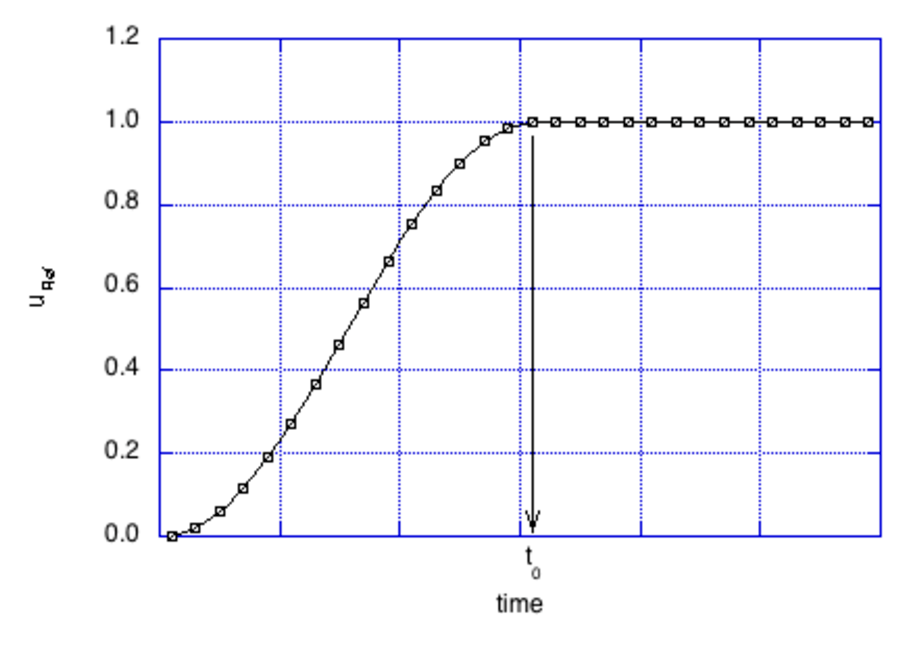
\includegraphics[width=7cm,clip]{accel_Velocity.eps}
\end{center}
\caption{加速中の速度プロファイル}
\label{fig:accel_velocity}
\end{figure}

%
\paragraph{時間積分幅$\Delta{t}$の指定}
\textbf{表\ref{tbl:delta t inc}}に時間積分幅\index{じかんせきぶんはば@時間積分幅}$\Delta{t}$の指定方法を示します.
拡散数\index{かくさんすう@拡散数}$D$は一次元の拡散方程式の場合$D=\alpha \delta t \slash h^2$で与えられます.$\alpha$は拡散係数で,Navier-Stokes方程式の場合$1/Re$,温度の輸送方程式の場合には$1/Pe$となります.安定性解析から$D<1 \slash 2$であることが要請されます.多次元の場合には,$d_m$を次元数として$\delta t<h^2 \slash (2d_m \alpha)$となります.

Delta\_tにはCFL数\index{CFL},または$\Delta t$を記述します.
時間積分幅の選択は,ソルバの種類を示すKind\_of\_Solverパラメータと関連があり,Solid\_Conductionの場合にはDt\_Directのみ選択できます.

\begin{table}[htdp]
\caption{Time\_Incrementのパラメータ指定}
\begin{center}
\small
\begin{tabular}{lll} \toprule
Dt\_Type & 時間積分幅の決定方法 & Delta\_tへの指定数値\\ \midrule
Direct & $\Delta t$を直接指定する & $\Delta t$\\
%CFL\_DFN\_MaxV & CFL\_MaxVと拡散数により制限される$\Delta t$の値の小さい方を選択\\
%CFL\_DFN\_RefV & CFL\_RefVと拡散数により制限される$\Delta t$の値の小さい方を選択\\
%CFL\_MaxV & CFL数を指定し,瞬時値の最大流速から$\Delta t$を決定 & CFL数\\
CFL\_Reference\_Velocity & CFL数を指定し,代表流速から$\Delta t$を決定 & CFL数\\
Diffusion & 拡散数から$\Delta t$を決定 & |\\
CFL\_Diffusion\_Reference\_Velocity & 代表流速に対するCFL数と拡散数から$\Delta t$を決定 & CFL数\\
%CFL\_MaxV\_CP & CFL数を指定し,音速を考慮した瞬時値の最大流速から$\Delta t$を決定 & CFL数\\
 \bottomrule
\end{tabular}
\end{center}
\label{tbl:delta t inc}
\end{table}

%
\pagebreak
\paragraph{計算時間の指定}
Period\_Typeで計算する時間の記述単位を指定します.
計算時間を時間で指定する場合,時間の単位は\hyperlink{tgt:unit}{Unit\_of\_Input\_Parameter}のモードに従います.
指定された単位の数値をCalculation\_Periodで指定します\footnote{SPHEREフレームワークでは,SPHERE定義要素としてCalculationStepsがありますが,内部的に上書きしています.}.

\end{indentation}



%%%
\pagebreak
\subsubsection{Treatment\_of\_Wall}

\hypertarget{tgt:treatment_of_wall}{壁面の扱い}について指定します.本パラメータは実験的実装です.

\begin{indentation}{3zw}{0zw}

{\small
\begin{program}
<Elem name="Treatment_of_Wall">
  <Param name="Pressure_Gradient" dtype="string" value="grad_zero"/>
  <Param name="Velocity_Profile"  dtype="string" value="no_slip"/>
</Elem>
\end{program}
}

各パラメータの意味について,\textbf{表\ref{tbl:wall_treatment}}に示します.
圧力勾配は法線方向の圧力勾配ゼロとNavier-Stokes方程式の圧力項を評価する2つの扱いが選択できます\footnote{現時点では,圧力勾配ゼロのみが選択できます.}.
速度プロファイルについては,滑りなし条件と壁関数を用いた近似が選択できます.壁関数は対数則が実装されています.詳細はCBCソルバークラス説明書をご覧ください\footnote{\today 未リリース.}.

\begin{table}[htdp]
\caption{壁面条件の指定}
\begin{center}
\small
\begin{tabular}{lll} \toprule
タグ & パラメータの値 & 説明\\ \midrule
Pressure\_Gradient & Grad\_Zero & 圧力勾配ゼロ\\
 & Grad\_NS & Navier-Stokes方程式から計算する\\ \hline
Velocity\_Profile  & No\_Slip & 滑りなし壁面条件\\
 & Slip & 滑り壁条件\\
 & Law\_of\_Wall & 壁法則\\ \bottomrule
\end{tabular}
\end{center}
\label{tbl:wall_treatment}
\end{table}

\end{indentation}


%%%
\pagebreak
\subsubsection{Unit}
\label{sec:p_unit}

入力ファイルと出力ファイルで用いる\hypertarget{tgt:unit}{単位を指定}します.

\begin{indentation}{3zw}{0zw}

{\small
\begin{program}
<Elem name="Unit">
  <Param name="Unit_of_Input_Parameter" dtype="STRING"  value="Dimensional" />
  <Param name="Pressure"                dtype="STRING"  value="gauge" />
  <Param name="Temperature"             dtype="STRING"  value="Celsius" />
</Elem>
\end{program}
}

各タグは,\textbf{表\ref{tbl:param_unit}}に示す単位の指定に用いられます.
有次元のファイル出力時には,圧力単位としてゲージ圧(Gauge Pressure)と絶対圧力(Absolute Pressure)が選択できます.
\textbf{式(\ref{eq:gauge pressure})}に示すゲージ圧を\textbf{式(\ref{eq:ND gauge})}により無次元化する場合に,基準圧として$p_0^\prime\,=\,1.0325\times 10^5$ [Pa]を用い,動圧が$10^0 \sim 10^3$程度とすると,$p \sim \mathrm{O}(1)$程度となるので,単精度計算では4桁程度有効桁が失われる場合もあります.
そのような場合,有次元値のファイル出力単位としてゲージ圧$p_g^\prime$を用います(非圧縮流れの場合には圧力差が意味をもつので,ゲージ圧でもかまいません).
ゲージ圧の基準となる大気圧$p_0^\prime\,$[Pa]は\hyperlink{tgt:reference}{Base\_Pressure}で指定します.
圧力単位の指定は,履歴ファイルのモニタ値にも適用されます.

\begin{equation}
p_g^\prime \,=\, p^\prime \,-\, p_0^\prime
\label{eq:gauge pressure}
\end{equation}

\begin{equation}
p \,=\, \frac{p_g^\prime}{\rho^\prime {u_0^\prime}^2}
\label{eq:ND gauge}
\end{equation}

\begin{table}[htdp]
\caption{単位の指定}
\begin{center}
\small
\begin{tabular}{lll} \toprule
タグ & 指定パラメータ & 説明\\ \midrule
Unit\_of\_Input\_Parameter & Dimensional or Non\_Dimensional & 入力パラメータファイルの単位を指定します(*1)\\
Pressure & Gauge or Absolute & 入力パラメータの単位が有次元のときに有効となります\\
Temperature & Celsius or Kelvin & 入力パラメータの単位が有次元のときに有効となります\\\bottomrule
\end{tabular}
\end{center}
\label{tbl:param_unit}
\end{table}

\end{indentation}



%%%
\pagebreak
\subsubsection{Version\_Info}

CBCソルバークラスとFlowBaseクラスの\hypertarget{tgt:version}{バージョン番号}を指定します.
異なる番号を指定している場合には,修正すべきバージョン番号が表示されるのでXMLファイルを変更します.

\begin{indentation}{3zw}{0zw}
\small
\begin{program}
<Elem name="Version_Info">
  <Param name="CBC"         dtype="INT"   value="127" />
  <Param name="Flow_Base"   dtype="INT"   value="225" />
</Elem>
\end{program}

\end{indentation}


%%%
\pagebreak
\subsubsection{VoxelDivisionMethod}
並列計算時の\hypertarget{tgt:voxel_division_method}{領域分割}をユーザーが明示的に指定します.直方体領域の計算空間を想定し,I, J, Kの各方向の分割数を指定します.
この指定が無い場合には,Sphereフレームワークがロードバランスが等しく,かつ通信面積が細小となる適切な分割を行います.

\begin{indentation}{3zw}{0zw}
\small
\begin{program}
<Elem name="VoxelDivisionMethod">
  <Param name="I"   dtype="INT"   value="8" />
  <Param name="J"   dtype="INT"   value="4" />
  <Param name="K"   dtype="INT"   value="5" />
</Elem>
\end{program}

\end{indentation}

%%% 隠しパラメータ
\begin{comment}
\subsubsection{Variable\_Range}

温度計算を実施する場合に,変数値を無次元値で[0,1]の範囲に\hypertarget{tgt:variable_range}{制限}することを指定します.

\begin{indentation}{3zw}{0zw}
\small

\begin{program}
<Param name="Variable_Range"     dtype="STRING" value="normal" />
\end{program}

\normalsize
温度の値に制限を課す場合に\textbf{表\ref{tbl:var_range}}に示すパラメータを使用します.保存則を満たさなくなるため,影響を考慮して利用してください.

\begin{table}[htdp]
\small
\caption{Variable\_Rangeのパラメータ指定}
\begin{center}
\begin{tabular}{ll} \toprule
タグ & モード\\ \midrule
cutoff & 値を無次元で[0, 1]に制限します\\
normal & 制限しません\\ \bottomrule
\end{tabular}
\end{center}
\label{tbl:var_range}
\end{table}

\end{indentation}
\end{comment}


%%%
\pagebreak
\subsection{Parameterセクション}
\label{sec:physical_parameter}

パラメータセクションでは,CBCソルバークラスの実行に必要な物理パラメータ\index{ぶつりぱらめーた@物理パラメータ}を記述します.



%%%
\subsubsection{Initial\_State}

\hypertarget{tgt:initial_state}{物理変数}の初期値\index{しょきち@初期値}を指定します.

\begin{indentation}{3zw}{0zw}

{\small
\begin{program}
<Elem name="Initial_State">
  <Param name="Density"     dtype="REAL" value="1.25e00" />
  <Param name="Pressure"    dtype="REAL" value="0.0" />
  <Param name="Temperature" dtype="REAL" value="20.0" />
  <Elem name="Velocity">
    <Param name="u" dtype="REAL" value="0.0"/>
    <Param name="v" dtype="REAL" value="0.0"/>
    <Param name="w" dtype="REAL" value="0.0"/>
  </Elem>
</Elem>
\end{program}
}

記述する初期値は有次元量で指定しますが,Solver\_Propertyセクションで\hyperlink{tgt:solver_property}{Kind\_of\_Solver}=\lq\lq Flow\_Only\rq\rq を指定した場合のみ,無次元での指定も可能です.
圧力値は,\hyperlink{tgt:unit}{Unit}で指定する圧力の単位に従います.
各変数の無次元化は以下のようになり,添え字の0は代表値または基準値を意味します.

\begin{equation}
\left.
\begin{array}{l}
\vspace{2mm}
\displaystyle{ \rho \,=\, \frac{\rho^{\prime}}{\rho_{0}^{\prime}} } \\
\vspace{2mm}
\displaystyle{ p \,=\, \frac{p^{\prime}-p_{0}^{\prime}}{\rho_{0}^{\prime}\,{u_{0}^{\prime}}^{2}} } \\
\vspace{2mm}
\displaystyle{ u_{i} \,=\, \frac{u_{i}^{\prime}}{u_0^{\prime}} } \\
\vspace{2mm}
\displaystyle{ \theta \,=\, \frac{\theta^{\prime}-\theta_{0}^{\prime}}{\Delta \theta^{\prime}} } 
\end{array} \qquad \right \}
\end{equation}

\end{indentation}

\vspace{3mm}
%%%
\subsubsection{Init\_Temp\_of\_Medium}
温度計算の場合に,割り当てた\hypertarget{tgt:initial_temp}{媒質}に対して初期温度を設定します.
媒質IDと流体・固体の種別は\hyperlink{tgt:model_setting}{Model\_Setting}と一致している必要があります.

{\small
\begin{program}
<Elem name="Init_Temp_of_Medium">
  <Param name="fluid" id="1"   dtype="real" value="20.0" />
  <Param name="solid" id="2"   dtype="real" value="34.0" />
  <Param name="solid" id="6"   dtype="real" value="34.0" />
  <Param name="solid" id="3"   dtype="real" value="35.0" />
  <Param name="fluid" id="4"   dtype="real" value="20.0" />
  <Param name="fluid" id="5"   dtype="real" value="20.0" />
  <Param name="fluid" id="10"  dtype="real" value="20.0" />
</Elem>
\end{program}
}

%%%
\pagebreak
\subsubsection{Intrinsic\_Example}

\hypertarget{tgt:intrinsic_example}{組み込み}例題\index{くみこみれいだい@組み込み例題}に固有のパラメータを指定します.

\begin{indentation}{3zw}{0zw}
\small

\begin{program}
<Elem name="Intrinsic_Example">
  ...
</Elem>
\end{program}

\normalsize
指定可能なパラメータは,\textbf{表\ref{tbl:intrinsic_parameter}}に示すように各\hyperlink{tgt:example}{組み込み例題}ごとに異なります.

\begin{table}[htdp]
\caption{Intrinsic\_Exampleセクションで指定できるパラメータ}
\begin{center}
\small
\begin{tabular}{llll} \toprule
組み込み例題 & 指定パラメータタグ & dtype & 指定値\\ \midrule
Duct3D & Shape     & STRING & Circular, Rectangular\\
       & Diameter  & REAL   & 断面径 [m]\\
       & Direction & STRING & X\_minus $|$ X\_plus $|$ Y\_minus $|$ Y\_plus $|$ Z\_minus $|$ Z\_plus\\
       & Driver    & REAL   & ドライバ部分の長さ [m]\\ \bottomrule
\end{tabular}
\end{center}
\label{tbl:intrinsic_parameter}
\end{table}

\end{indentation}



%%%
\pagebreak
\subsubsection{Reference}

解析に用いる無次元化の\hypertarget{tgt:reference}{基準量},あるいは無次元パラメータを指定します.

\begin{indentation}{3zw}{0zw}

{\small
\begin{program}
<Elem name="Reference">
  <Param name="Length"        dtype="REAL" value="1.0" />
  <Param name="Velocity"      dtype="REAL" value="1.0" />
  <Param name="Base_Pressure" dtype="REAL" value="101325" />
  <Param name="Gravity"       dtype="REAL" value="9.8" />
  <Param name="Reynolds"      dtype="REAL" value="1000.0" />
  <Param name="Prandtl"       dtype="REAL" value="0.71" />
  <Param name="Ref_ID"        dtype="INT"  value="1" />
</Elem>
\end{program}
}

\noindent \textbf{表\ref{tbl:ref_value}}に示すように基準量を必要に応じて記述できます.
無次元パラメータであるReynolds数とPrandtl数は,\hyperlink{tgt:unit}{Unit}の指定が無次元のときのみ指定できます.
Ref\_IDで指定するIDは,ボクセルモデル内で使われ,かつ\hyperlink{tgt:model_setting}{Model\_Setting}セクションで記述されている必要があります.固体熱伝導解析の場合には固体のIDを指定し,それ以外の(熱)流動解析の場合には流体のIDを指定します.

\begin{table}[htdp]
\caption{Referenceセクションで指定できるパラメータ}
\begin{center}
\small
\begin{tabular}{llll} \toprule
値 & 意味 & 単位\\ \midrule
Length & 代表長さ & $m$ &\\
Velocity & 代表速度 & $m/s$ &\\
Base\_Pressure & 基準圧力 & $Pa$ &\\
Gravity & 重力加速度 & $m^2/s$ &\\
%Grashof & グラショフ数 & |\\
Prandtl & プラントル数 & | & 無次元のときのみ指定\\
%Rayleigh & レイリー数 & |\\
Reynolds & レイノルズ数 & | & 無次元のときのみ指定\\
Ref\_ID & 代表物性値として指定する媒質ID & | &\\ \bottomrule
\end{tabular}
\end{center}
\label{tbl:ref_value}
\end{table}

\end{indentation}



%%%
\pagebreak
\subsubsection{Temperature}

\hypertarget{tgt:temperature}{温度計算}を実施する場合の基準量を有次元値で指定します.

\begin{indentation}{3zw}{0zw}

{\small
\begin{program}
<Elem name="Temperature">
  <Param name="Base"       dtype="REAL"   value="293.15" />
  <Param name="Difference" dtype="REAL"   value="35.0" />
</Elem>
\end{program}
}

基準温度(Base)と温度差(Difference)は,非圧縮計算のパッシブスカラーによる温度計算では温度場を特徴づける代表量となります.
単位は\hyperlink{tgt:unit}{Temperature}タグで指定します.

\end{indentation}



%%%
\pagebreak
\subsection{Medium\_Tableセクション}

ソルバーで利用する媒質の\hypertarget{tgt:medium_table}{物性値テーブル}を記述します.
ここで記述する媒質の基本リスト\index{きほんりすと@基本リスト!ばいしつの@媒質の---}は,解析に利用される候補です.
媒質は流体と固体が記述でき,\textbf{表\ref{tbl:MTLentry}}により媒質を指定します.

\begin{indentation}{3zw}{0zw}

{\small
\begin{program}
<Medium_Table>
  <Elem name="Fluid" id="100" comment="Air">
    <Param name="density"              dtype="REAL" value="1.1763" />
    <Param name="specific_heat"        dtype="REAL" value="1007" />
    <Param name="thermal_conductivity" dtype="REAL" value="2.614e-02" />
    <Param name="kinematic_viscosity"  dtype="REAL" value="15.83e-06" />
    <Param name="viscosity"            dtype="REAL" value="18.62e-06" />
    <Param name="sound_of_speed"       dtype="REAL" value="340.0" />
    <Param name="volume_expansion"     dtype="REAL" value="0.04e-3" />
  </Elem>
  <Elem name="Solid" id="600" comment="Fe">
    <Param name="density"              dtype="REAL" value="7870.0" />
    <Param name="specific_heat"        dtype="REAL" value="442.0" />
    <Param name="thermal_conductivity" dtype="REAL" value="80.3" />
  </Elem>
</Medium_Table>
\end{program}
}

\begin{table}[htdp]
\caption{Medium\_Tableに記述するパラメータ}
\begin{center}
\begin{tabular}{ll} \toprule
タグ & 説明\\ \midrule
Elem name & Fluid または Solid\\
ID & 媒質ID\\
comment & 媒質名\\ \bottomrule
\end{tabular}
\end{center}
\label{tbl:MTLentry}
\end{table}


各媒質は固体と流体によって記述しなければならない物性値が異なります.
指定できる項目を\textbf{表\ref{tbl:medium_tbl}}に示します.
固体については,密度・比熱・熱伝導率のみの記述となります.
各媒質の情報は,任意に指定するID番号によって管理されます.

\begin{table}[htdp]
\caption{Medium\_Tableにおける物性値の指定}
\begin{minipage}{.45\textwidth}
\begin{center}
\begin{tabular}{lll}\\ \toprule
Fluidのキーワード & 説明 & 単位\\ \midrule
Density & 密度 & $kg/m^3$\\
Specific\_Heat & 定圧比熱 & $kJ/(kg K)$\\
Thermal\_Conductivity & 熱伝導率 & $W/(m K)$\\
Kinematic\_Viscosity & 動粘性係数 & $m^2/s$\\
Viscosity & 粘性係数 & $Pa\,s$\\
Sound\_of\_Speed & 音速 & $m/s$\\
Volume\_Expansion & 体膨張率 & $1/K$\\ \bottomrule
\end{tabular}
\end{center}
\end{minipage} \hfill
\begin{minipage}{.45\textwidth}
\begin{center}
\begin{tabular}{lll}\\ \toprule
Solidのキーワード & 説明 & 単位\\ \midrule
Density & 密度 & $kg/m^3$\\
Specific\_Heat & 定圧比熱 & $kJ/(kg K)$\\
Thermal\_Conductivity & 熱伝導率 & $W/(m K)$\\ \bottomrule
\end{tabular}
\end{center}
\end{minipage}
\label{tbl:medium_tbl}
\end{table}

\end{indentation}

